% =====================================================================
%  CAPÍTULO I — FUNDAMENTAÇÃO TEÓRICA
%
%  Revisado em 2026-10-05, a pedido do autor: o escopo é ARIMA, ARIMA-GARCH
%  e as médias móveis de Almeida (2016). Saíram os indicadores que o
%  trabalho não usa (IFR, MME, Bandas de Bollinger, MACD) e tudo o que era
%  de aprendizado de máquina (LSTM, SARIMA, integração com Python). A
%  versão anterior está em notas/rascunhos/antes_revisao_2026-10-05/.
%
%  Títulos só com a inicial maiúscula (Manual FATEC-ID, item 4.1.2.10).
%
%  Varredura do autor em 2026-10-15: figuras fixas no lugar ([H]); "pregão"
%  definido; ADF (raiz unitária e valor-p) e AIC explicados com Thomaz (2019,
%  p. 28, 40-41, 44-45); ARMA e AR como casos do ARIMA (Thomaz, 2019, p. 33);
%  citação dupla "(Xing; Araya; Araya)" virou narrativa; frase do agrupamento
%  de volatilidade reescrita; saiu a remissão às considerações finais; as três
%  formas de usar o GARCH foram para o Cap. II (decisão de projeto, sem fonte);
%  "Medidas de desempenho e risco" virou "Métricas de avaliação", com quadro de
%  todas as métricas e a explicação da raiz de 252 (Sharpe, 1994, regra da raiz
%  do tempo; 252 = convenção, marcado para fonte; média de 247,8 pregões/ano em
%  dados/series/PETR4_OFICIAL.csv). Equações sem rótulo: o texto não as cita
%  mais pelo número. Versão anterior em
%  notas/rascunhos/antes_varredura_autor_2026-10-15/.
% =====================================================================
\setdiv{CAPÍTULO I}
\chapter{Fundamentação teórica}

Este capítulo reúne os conceitos sobre os quais o trabalho se apoia. Parte do
ambiente em que as operações acontecem, isto é, a bolsa de valores e a plataforma
de negociação, passa pela análise técnica e pelas médias móveis empregadas por
\citeonline{almeida2016} e chega aos modelos estatísticos ARIMA e GARCH e às medidas usadas para avaliar uma estratégia. Ao
final, são apresentados os trabalhos relacionados.

\section{Mercado de ações}

De acordo com o \citeonline{bcbBolsas}, as bolsas de valores são sociedades
anônimas ou associações civis que mantêm local ou sistema adequado à realização de
operações de compra e venda de títulos e valores mobiliários, em mercado livre e
aberto, organizado e fiscalizado por seus membros e pela Comissão de Valores
Mobiliários. No Brasil, esse papel é exercido pela B3.

Para a empresa, a abertura de capital é uma forma de obter recursos de terceiros.
Em troca do capital recebido, ela cede aos acionistas uma participação no negócio
proporcional ao valor investido. Para o investidor, a ação passa a ser um ativo
cujo preço varia a cada pregão, isto é, a cada sessão diária de negociação na
bolsa, conforme a oferta e a procura, e é essa variação
que as estratégias de negociação procuram aproveitar.

O investidor não negocia diretamente na bolsa. O acesso se dá por meio de
corretoras, instituições que intermediam as operações e oferecem serviços como
plataformas de negociação pela internet, custódia dos títulos e financiamento para
a compra de ações, cobrando por isso comissões e taxas \cite{bcbCorretoras}. É
pela corretora que uma plataforma como o MetaTrader 5 se conecta ao mercado.

Toda decisão de investimento envolve um compromisso entre risco e retorno, uma vez
que os recursos são limitados e precisam ser distribuídos entre alternativas
\cite{elder2002}. No Brasil, a principal referência para essa comparação é a taxa
Selic, a taxa básica de juros da economia, que serve de base para as demais taxas
praticadas no mercado e influencia tanto o custo do crédito quanto o retorno das
aplicações financeiras \cite{bcbSelic}. Por esse motivo, o capital que uma
estratégia mantém fora do mercado costuma ser comparado ao que renderia se
estivesse aplicado a essa taxa.

\section{Análise técnica}

A análise técnica busca antecipar o comportamento dos preços a partir do estudo do
seu próprio histórico, procurando padrões e tendências que possam indicar o
movimento seguinte. Sua origem remonta ao comércio de arroz, e hoje ela é aplicada
a ações, moedas e outros ativos. Para essa abordagem, o que importa é o
comportamento do preço, sem considerar notícias ou outros fatores que possam
influenciar o mercado \cite{fernandes2014}.

\citeonline{fernandes2014} distingue duas vertentes. A empírica, ou clássica, é a
mais antiga: o analista observa o gráfico e identifica tendências, suportes,
resistências e padrões que, segundo essa abordagem, tendem a se repetir. Por
depender da interpretação de quem observa, ela é sujeita a conclusões diferentes
sobre o mesmo ativo. A estatística, ou moderna, substitui a interpretação visual
por cálculos aplicados à série de preços, o que torna a análise reproduzível e
permite que ela seja executada por um programa de computador.

É na segunda vertente que este trabalho se insere. Tanto a estratégia de médias
móveis de \citeonline{almeida2016} quanto os modelos ARIMA e GARCH são regras
matemáticas aplicadas ao histórico de preços, e por isso podem ser programados,
testados sobre dados passados e comparados entre si sob as mesmas condições.

\subsection{Médias móveis}

A média móvel é um dos instrumentos mais utilizados da análise técnica. Ela
calcula o preço médio de um ativo nos últimos $n$ períodos e é recalculada a cada
novo período, descartando o valor mais antigo e incorporando o mais recente. Com
isso, suaviza as oscilações de curto prazo e evidencia a direção predominante dos
preços \cite{fernandes2014}. Na média móvel simples, todos os preços da janela
recebem o mesmo peso, de modo que a média de dez períodos atribui peso de um
décimo a cada um dos dez últimos fechamentos.

O tamanho da janela determina o comportamento da média. Janelas curtas reagem
rapidamente a mudanças de preço, mas produzem mais sinais falsos, enquanto janelas
longas filtram melhor o ruído, à custa de reconhecer uma nova tendência com
atraso \cite{fernandes2014}. A estratégia de cruzamento combina as duas: utiliza
uma média rápida, de janela curta, e uma lenta, de janela longa, e interpreta o
cruzamento entre elas como sinal de compra ou de venda, como ilustra a
Figura~\ref{fig:cruzamento-mm}.

\begin{figure}[H]
\centering
\caption{Cruzamento de médias móveis}
\label{fig:cruzamento-mm}
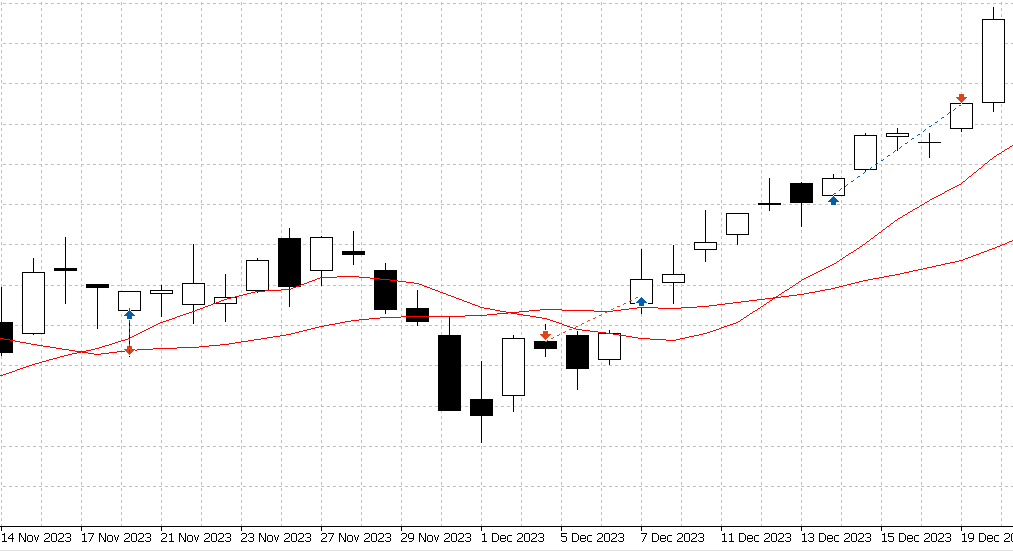
\includegraphics[width=0.8\textwidth]{fig04-cruzamento-medias.png}
\fonte{Elaboração própria com dados e interface do MetaTrader 5.}
\end{figure}

Foi essa a estratégia adotada por \citeonline{almeida2016}. O autor utilizou duas
médias móveis simples, uma de dez e outra de vinte períodos, calculadas sobre o
preço de fechamento, e operou nos dois sentidos, comprando quando a média rápida
cruzava a lenta para cima e vendendo no cruzamento inverso. Seu algoritmo previa
ainda parâmetros de limite de perda e de realização de lucro, embora os testes
relatados tenham sido conduzidos com ambos nulos. O próprio autor alertou para as
limitações de se usar apenas essa técnica em mercados de alta volatilidade
\cite{almeida2016}.

\section{MetaTrader 5}

O MetaTrader 5 é uma plataforma de negociação multimercado desenvolvida pela
MetaQuotes, que reúne em um mesmo ambiente a execução de ordens, a análise gráfica
e o desenvolvimento de sistemas automatizados para ações, futuros, moedas e outros
instrumentos \cite{metaquotes2024}. Sua interface, mostrada na
Figura~\ref{fig:interface-mt}, organiza em janelas as cotações em tempo real, os
gráficos de preços e o navegador, que dá acesso às contas, aos indicadores e aos
programas instalados.

\begin{figure}[H]
\centering
\caption{Interface do MetaTrader 5}
\label{fig:interface-mt}
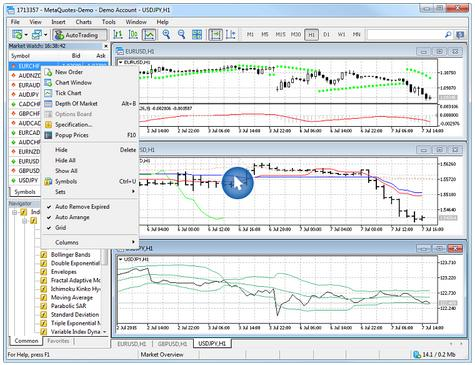
\includegraphics[width=0.72\textwidth]{fig01-interface-metatrader.png}
\fonte{\citeonline{metaquotes2024}.}
\end{figure}

Os programas que negociam de forma automática na plataforma são chamados de
\textit{Expert Advisors} (EAs), também conhecidos como robôs de negociação. Um EA
abre, modifica e encerra posições segundo regras programadas, sem intervenção
manual \cite{almeida2016}. A Figura~\ref{fig:fluxograma-ea} apresenta o ciclo de
funcionamento de um EA.

\begin{figure}[H]
\centering
\caption{Ciclo de funcionamento de um \textit{Expert Advisor}}
\label{fig:fluxograma-ea}
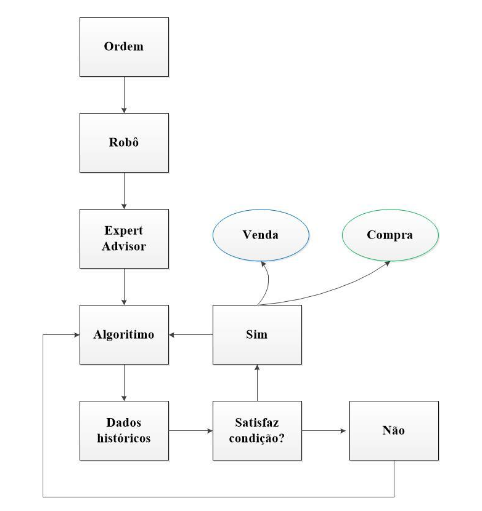
\includegraphics[width=0.42\textwidth]{fig02-fluxograma-ea.png}
\fonte{\citeonline{almeida2016}.}
\end{figure}

Os EAs são escritos em MQL5, linguagem própria da plataforma, de sintaxe próxima à
do C++. O ambiente de desenvolvimento, chamado MetaEditor, oferece editor,
compilador e depurador integrados. Para avaliar uma estratégia antes de usá-la, a
plataforma dispõe do testador de estratégias, o \textit{Strategy Tester}, que
executa o EA sobre dados históricos, simulando as ordens como se o mercado
estivesse aberto, e produz relatórios de desempenho \cite{metaquotes2024}. Esse
procedimento é conhecido como \textit{backtesting}, e foi por meio dele que todos
os experimentos deste trabalho foram conduzidos.

\section{Modelos estatísticos de séries temporais}

Uma série temporal é uma sequência de observações ordenadas no tempo, como os
preços de fechamento diários de uma ação. Os modelos de séries temporais procuram
descrever a estrutura dessa sequência, isto é, de que forma cada observação se
relaciona com as anteriores, e utilizam essa descrição para projetar valores
futuros. Neste trabalho são empregados dois desses modelos, com funções
diferentes. O ARIMA descreve o valor esperado da série, e o GARCH descreve o
tamanho esperado dos erros em torno desse valor.

\subsection{ARIMA}

O modelo autorregressivo integrado de médias móveis, conhecido pela sigla ARIMA,
do inglês \textit{Autoregressive Integrated Moving Average}, é um dos modelos mais
empregados na previsão de séries temporais, inclusive em séries financeiras
\cite{xing2024}. Ele é composto por três partes, cada uma associada a uma ordem.

A parte autorregressiva, de ordem $p$, expressa o valor atual da série como
combinação dos seus $p$ valores anteriores. A parte de médias móveis, de ordem
$q$, acrescenta a influência dos $q$ erros de previsão anteriores, isto é, das
diferenças entre o que o modelo previu e o que de fato ocorreu. A parte integrada,
de ordem $d$, indica quantas vezes a série precisa ser diferenciada, ou seja,
substituída pela variação entre uma observação e a anterior, para se tornar
estacionária \cite{xing2024}. Uma série é estacionária quando sua média e sua
variância não se alteram ao longo do tempo, condição exigida pelas partes
autorregressiva e de médias móveis.

Convém registrar que a média móvel do ARIMA não é a mesma média móvel da análise
técnica. Na análise técnica, a média é calculada sobre os preços. No ARIMA, o
termo de médias móveis é uma combinação dos erros de previsão passados. Os dois
conceitos têm o mesmo nome, mas descrevem coisas diferentes.

Representando por $y_t$ a série já diferenciada $d$ vezes, o modelo pode ser
escrito como
\begin{equation}
y_t = c + \phi_1 y_{t-1} + \cdots + \phi_p y_{t-p}
        + \varepsilon_t + \theta_1 \varepsilon_{t-1} + \cdots + \theta_q \varepsilon_{t-q},
\end{equation}
em que $c$ é uma constante, os coeficientes $\phi$ ponderam os valores passados da
série, os coeficientes $\theta$ ponderam os erros passados e $\varepsilon_t$ é o
erro do período atual, que o modelo não consegue prever.

O ARIMA supõe, portanto, que a série diferenciada segue um modelo ARMA($p$,$q$),
que tem apenas as partes autorregressiva e de médias móveis \cite{thomaz2019}.
Quando a série não precisa ser diferenciada ($d = 0$), o próprio ARIMA é um ARMA,
e quando também não há termos de médias móveis ($q = 0$), o modelo é chamado de
AR($p$), ou autorregressivo.

Há uma relação direta entre essa equação e a estratégia de
\citeonline{almeida2016}. A média móvel simples de dez períodos é um filtro linear
que atribui pesos fixos, iguais a um décimo, aos últimos preços. A parte
autorregressiva do ARIMA também é um filtro linear sobre os valores passados, mas
seus pesos $\phi$ são estimados a partir dos dados, em vez de fixados por
convenção. Nesse sentido, o ARIMA pode ser visto como uma generalização da média
móvel: mantém a mesma família de operação e ajusta os coeficientes ao ativo e ao
período analisados.

A aplicação do modelo segue as etapas representadas na
Figura~\ref{fig:fluxo-arima}.

\begin{figure}[H]
\centering
\caption{Etapas de aplicação do modelo ARIMA}
\label{fig:fluxo-arima}
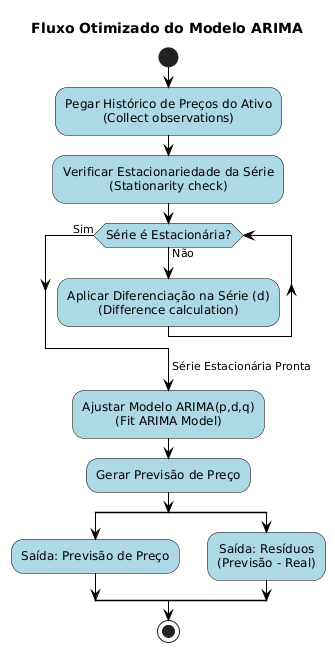
\includegraphics[width=0.4\textwidth]{fig05-fluxo-arima.png}
\fonte{Elaboração própria.}
\end{figure}

A primeira etapa é verificar se a série é estacionária. Uma série estacionária
oscila em torno de uma média estável, e um choque que a afasta dessa média tende a
se desfazer com o tempo. Os preços de ações, ao contrário, costumam se comportar
como um passeio aleatório, em que cada choque se incorpora ao preço e não se
desfaz, de modo que a variância da série cresce com o tempo \cite{thomaz2019}.
Esse comportamento é chamado de raiz unitária. Para identificá-lo, usa-se o teste
de Dickey-Fuller aumentado (ADF), que estima, por regressão, o quanto a variação de
cada dia depende do nível da série no dia anterior. Se a série tende a voltar à
sua média, essa dependência é negativa e forte. Se não tende, ela é próxima de
zero, e a série tem raiz unitária \cite{thomaz2019}.

A hipótese nula do teste é a existência de raiz unitária. O valor-p indica a
probabilidade de se obter um resultado tão favorável à estacionariedade quanto o
observado se a série de fato tivesse raiz unitária. Como a estatística do teste não
segue as distribuições usuais, os seus valores críticos foram tabelados
especialmente para ele, e a hipótese nula é rejeitada quando a estatística fica
abaixo do valor crítico, o que corresponde a um valor-p pequeno, em geral menor
que 0,05 \cite{thomaz2019}. Quando a hipótese não é rejeitada, a série é
diferenciada e testada de novo. No estudo de \citeonline{xing2024} sobre as ações
da NVIDIA, o teste aplicado aos preços resultou em valor-p de 0,998773, isto é, sem
nenhum indício contra a raiz unitária. Após uma diferenciação, o valor-p ficou
próximo de zero, e a ordem de integração foi definida como $d = 1$.

Definido $d$, resta escolher $p$ e $q$. Como várias combinações são possíveis,
\citeonline{xing2024} testaram valores de zero a quatro para cada ordem e
escolheram a combinação de menor critério de informação de Akaike (AIC), dado por
\begin{equation*}
\text{AIC} = -2\ln \hat{L} + 2k,
\end{equation*}
em que $\hat{L}$ é a verossimilhança do modelo ajustado, que mede o quão provável é
a série observada segundo o modelo, e $k$ é o número de parâmetros estimados
\cite{thomaz2019}. A primeira parcela diminui quanto melhor o ajuste, e a segunda
aumenta a cada parâmetro acrescentado. Um modelo com mais parâmetros sempre se
ajusta um pouco melhor aos dados passados, mas parte desse ganho é apenas ruído
reproduzido, que não ajuda a prever. A penalidade faz com que um parâmetro a mais
só compense se melhorar o ajuste mais do que custa. Ajusta-se, então, cada
combinação candidata, e escolhe-se a de menor AIC, que é a que melhor equilibra
ajuste e simplicidade. Com o modelo escolhido, obtêm-se a previsão para o período
seguinte e os resíduos, que são os erros de previsão observados na amostra.

Segundo \citeonline{xing2024} e \citeonline{araya2024}, a principal limitação do
ARIMA é tratar apenas relações lineares e supor que a variância dos erros é
constante. Em séries financeiras essa segunda suposição raramente se verifica, e é
dela que trata o modelo GARCH.

\subsection{GARCH}

Nas séries de retornos de ações, a volatilidade, que mede o grau de variação dos
preços ao longo do tempo, não é constante. Ela costuma vir em ondas, com dias
agitados seguidos de outros dias agitados e dias calmos seguidos de dias calmos, e
conhecê-la é fundamental para a gestão de risco \cite{araya2024}.
\citeonline{engle1982} propôs o modelo ARCH, em que a variância do erro de cada
período depende dos erros dos períodos anteriores. \citeonline{bollerslev1986}
generalizou essa proposta no modelo GARCH, do inglês \textit{Generalized
Autoregressive Conditional Heteroskedasticity}, em que a variância passa a
depender também das próprias variâncias anteriores.

Na especificação GARCH(1,1), adotada neste trabalho, a variância condicional
$\sigma^2_t$ do erro no período $t$ é dada por
\begin{equation}
\sigma^2_t = \omega + \alpha\,\varepsilon^2_{t-1} + \beta\,\sigma^2_{t-1},
\end{equation}
em que $\varepsilon_{t-1}$ é o erro do período anterior, $\sigma^2_{t-1}$ é a
variância estimada para o período anterior e $\omega$, $\alpha$ e $\beta$ são os
parâmetros do modelo. O termo com $\alpha$ representa a reação da volatilidade a
um choque recente, e o termo com $\beta$ representa a persistência da
volatilidade passada \cite{bollerslev1986}. A Figura~\ref{fig:fluxo-garch}
ilustra esse processo de retroalimentação.

\begin{figure}[H]
\centering
\caption{Retroalimentação da variância no modelo GARCH}
\label{fig:fluxo-garch}
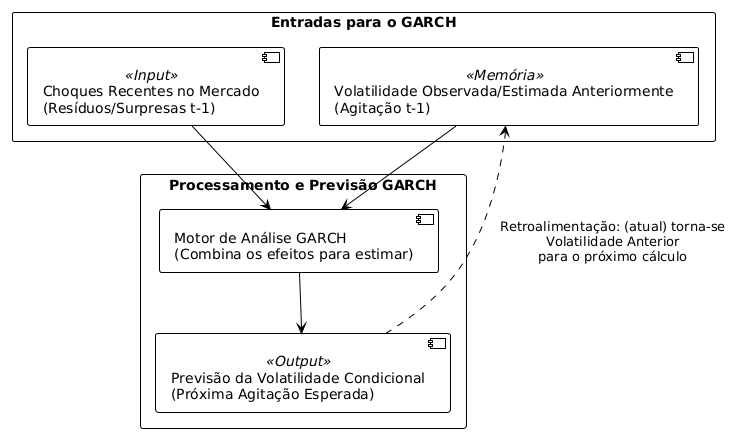
\includegraphics[width=0.7\textwidth]{fig06-fluxo-garch.png}
\fonte{Elaboração própria.}
\end{figure}

Para que o modelo faça sentido, os parâmetros precisam respeitar restrições:
$\omega$ deve ser positivo, $\alpha$ e $\beta$ não podem ser negativos e a soma
$\alpha + \beta$ deve ser menor que um. A última condição garante que a
variância tenha um valor de longo prazo finito, igual a
$\omega / (1 - \alpha - \beta)$, para o qual a volatilidade retorna depois de um
choque \cite{bollerslev1986}.

O GARCH padrão trata de forma simétrica os choques positivos e os negativos de
mesma magnitude. Nos mercados de ações, porém, as quedas costumam elevar a
volatilidade mais do que as altas. Para representar essa assimetria foram
propostas variações do modelo, como o EGARCH e o TGARCH, que acrescentam à
equação termos capazes de fazer a volatilidade reagir de forma diferente a
choques positivos e negativos \cite{araya2024}. Este trabalho emprega a
especificação simétrica.

\subsection{Integração entre ARIMA e GARCH}

Os dois modelos se complementam. O ARIMA estima a média condicional da série, ou
seja, o valor esperado para o período seguinte. O GARCH estima a variância
condicional dos erros desse valor esperado. Na forma combinada, os resíduos
gerados pelo ARIMA servem de entrada para o GARCH, que modela a variância desses
resíduos ao longo do tempo \cite{araya2024}.

Em uma estratégia de negociação, essa combinação permite separar duas perguntas. A
direção da operação é dada pelo sinal da previsão do ARIMA, e o risco associado a
ela é dado pela volatilidade prevista pelo GARCH. Como o GARCH não fornece nenhuma
informação sobre a direção dos preços, ele não pode, sozinho, gerar uma ordem de
compra ou de venda. O que ele pode fazer é condicionar a operação indicada pelo
ARIMA ao nível de risco esperado, impedindo a operação ou reduzindo o seu tamanho
quando a volatilidade prevista é alta.

\section{Métricas de avaliação}
\label{sec:medidas}

Avaliar uma estratégia de negociação apenas pelo lucro final esconde o caminho
percorrido até ele. Duas estratégias com o mesmo retorno podem ter exposto o
investidor a riscos muito diferentes. Por isso, o relatório do testador de
estratégias do MetaTrader 5 apresenta, ao lado do lucro, medidas de risco e
índices que relacionam as duas coisas \cite{metaquotesRelatorio}. O
Quadro~\ref{qua:metricas} resume as métricas usadas neste trabalho para avaliar e
comparar os robôs.

\begin{quadro}[H]
\centering
\caption{Métricas de avaliação usadas no trabalho}
\label{qua:metricas}
\fontsize{10}{12}\selectfont
\begin{tabular}{|>{\raggedright\arraybackslash}p{3.0cm}|>{\raggedright\arraybackslash}p{5.2cm}|>{\raggedright\arraybackslash}p{6.2cm}|}
\hline
Métrica & O que indica & Como é calculada \\
\hline
Retorno acumulado & quanto o patrimônio cresceu ou diminuiu no período & patrimônio final dividido pelo inicial, menos um \\
\hline
Queda máxima & o pior tombo que um investidor teria sofrido seguindo a estratégia & maior queda percentual do patrimônio entre um ponto alto e o ponto mais baixo seguinte \\
\hline
Volatilidade & o quanto o patrimônio sobe e desce de um dia para o outro & desvio-padrão dos retornos diários do patrimônio, em base anual \\
\hline
Negociações & quantas operações o robô realizou & contagem do relatório do testador \\
\hline
Taxa de acerto & a proporção de negociações que terminaram com lucro & negociações com lucro divididas pelo total \\
\hline
Sinais vetados & quantas vezes o GARCH impediu uma operação indicada pelo ARIMA & contagem registrada pelo robô \\
\hline
Índice de Sharpe & o ganho além de uma referência por unidade de oscilação & média do retorno diferencial dividida pelo seu desvio-padrão \\
\hline
Índice de Calmar & o ganho por unidade de queda máxima & retorno anualizado dividido pela queda máxima \\
\hline
\end{tabular}
\fonte{Elaboração própria, com base em \citeonline{metaquotesRelatorio} e \citeonline{sharpe1994}.}
\end{quadro}

O risco é medido de duas formas complementares. A queda máxima, que o relatório
da plataforma chama de rebaixamento relativo e que também é conhecida pelo termo em
inglês \textit{drawdown}, é a maior queda percentual entre um máximo local do
patrimônio e o mínimo local seguinte \cite{metaquotesRelatorio}. Ela responde à
pergunta de qual foi o pior tombo do caminho. A volatilidade, por sua vez, é o
desvio-padrão dos retornos e mede o quanto o patrimônio oscila no dia a dia.

Como os retornos são diários, a volatilidade é convertida para base anual, o que
facilita a leitura e a comparação. Se os retornos de dias diferentes forem
independentes entre si, a variância de um período de $T$ dias é $T$ vezes a
variância diária, e o desvio-padrão, a raiz de $T$ vezes o diário
\cite{sharpe1994}. Usou-se $T = 252$, número de dias úteis de um ano adotado por
convenção no mercado brasileiro. Na série da PETR4 usada neste trabalho, a média
foi de 248 pregões por ano. A volatilidade anual é, portanto, o desvio-padrão
diário multiplicado pela raiz de 252, e uma oscilação típica de 2\% ao dia
corresponde a cerca de 32\% ao ano.
% REFERÊNCIA (convenção de 252 dias úteis, a buscar): Banco Central do Brasil,
% taxa Selic anualizada com base 252. A média de 247,8 pregões por ano (2004 a
% 2025) sai de dados/series/PETR4_OFICIAL.csv.

O índice de Sharpe relaciona o retorno de uma estratégia à sua volatilidade. Ele
divide o retorno diferencial, isto é, a diferença entre o retorno da estratégia e
o de uma referência, pelo desvio-padrão dessa diferença \cite{sharpe1994},
\begin{equation}
S = \frac{\bar{d}}{\sigma_d},
\end{equation}
em que $\bar{d}$ é a média do retorno diferencial e $\sigma_d$ o seu
desvio-padrão. O índice indica quanto se ganhou além da referência por unidade de
oscilação, e quanto maior, melhor a relação. Um índice negativo indica que a
estratégia rendeu menos que a referência. O testador do MetaTrader 5 usa como
referência um rendimento livre de risco igual a zero \cite{metaquotesRelatorio}, e
neste trabalho a referência foi a taxa Selic. O próprio autor observa que o
índice está ligado à estatística $t$ da média do retorno diferencial, que é igual
a ele multiplicado pela raiz do número de observações \cite{sharpe1994}. Por isso,
um mesmo valor de índice é estatisticamente mais forte quando medido em um período
mais longo.

O índice de Calmar relaciona o retorno à queda máxima. Ele divide o retorno
anualizado pela queda máxima do período,
\begin{equation}
C = \frac{\text{retorno anualizado}}{\text{queda máxima}},
\end{equation}
e segue a mesma ideia do fator de recuperação do relatório da plataforma, que
divide o lucro obtido pelo rebaixamento máximo \cite{metaquotesRelatorio}, com a
diferença de usar o retorno anualizado, o que permite comparar períodos de
durações diferentes. O índice indica quanto se ganhou por unidade do pior tombo e,
por isso, favorece estratégias que evitam perdas grandes. Os dois índices medem
coisas diferentes. O Sharpe penaliza toda oscilação, para cima ou para baixo, e o
Calmar considera apenas a pior queda.

\section{Trabalhos relacionados}

Os trabalhos relacionados foram selecionados entre pesquisas sobre o
desenvolvimento de robôs de negociação na plataforma MetaTrader 5 e sobre a
aplicação dos modelos ARIMA e GARCH à previsão de séries de preços de ações.

O estudo de \citeonline{almeida2016}, desenvolvido na FATEC Indaiatuba, é o ponto
de partida deste trabalho. O autor desenvolveu em MQL5 um robô de negociação para
a PETR4 baseado no cruzamento de médias móveis simples de dez e vinte períodos e o
avaliou por \textit{backtesting} em períodos de crise, entre 2007 e 2011, e fora
de crise, entre 2013 e 2016. A estratégia apresentou lucro no período fora de
crise e prejuízo no período de crise. Ao discutir os limites do
trabalho, o autor indicou a investigação de modelos de volatilidade, entre eles o
GARCH, como continuidade da pesquisa. É essa indicação que o presente trabalho
retoma, mantendo o ativo, a plataforma e a linguagem.

\citeonline{batista2024} também desenvolveu um \textit{Expert Advisor} em MQL5
para a B3, combinando três indicadores técnicos, a média móvel exponencial, a
convergência e divergência de médias móveis e o índice de força relativa. Os testes,
realizados sobre o ativo BBAS3F em 2023, compararam os indicadores isoladamente,
em pares e em conjunto, e a combinação dos três apresentou o melhor resultado. O
estudo mostra que a integração de técnicas com funções distintas em um mesmo
algoritmo pode melhorar a decisão, ideia que este trabalho aplica aos modelos
estatísticos.

\citeonline{xing2024} compararam o ARIMA, o ARIMA-GARCH e dois modelos de redes
neurais na previsão do preço de fechamento das ações da NVIDIA, com dados diários
de abril de 2019 a abril de 2024. As ordens dos modelos ARIMA foram definidas pelo
teste ADF e pelo menor AIC, com $p$ e $q$ variando de zero a quatro, procedimento
semelhante ao adotado neste trabalho. O ARIMA-GARCH apresentou a menor raiz do erro
quadrático médio, e o ARIMA com janela expansiva teve o melhor desempenho geral,
superando as redes neurais. Os autores atribuem esse resultado, possivelmente, ao
comportamento predominantemente linear da série.

\citeonline{araya2024} estudaram a previsão da volatilidade das ações da Apple.
No modelo proposto, os resíduos de um modelo SARIMA, versão do ARIMA com
componentes sazonais, alimentam um modelo GARCH, e a volatilidade estimada por essa combinação é depois utilizada como
entrada de redes neurais. A etapa que interessa a este trabalho é a primeira, em
que os resíduos do modelo de média servem de entrada para o modelo de variância,
mesma arquitetura adotada no algoritmo aqui desenvolvido.

O Quadro~\ref{qua:comparativa} resume as características desses estudos e as
deste trabalho.

\begin{quadro}[H]
\centering
\caption{Características dos estudos relacionados}
\label{qua:comparativa}
\fontsize{10}{12}\selectfont
\begin{tabular}{|>{\raggedright\arraybackslash}p{2.6cm}|>{\raggedright\arraybackslash}p{2.2cm}|>{\raggedright\arraybackslash}p{2.5cm}|>{\raggedright\arraybackslash}p{2.1cm}|>{\raggedright\arraybackslash}p{4.0cm}|}
\hline
Estudo & Ativo & Fonte de dados & Periodicidade & Método \\
\hline
\citeonline{almeida2016} & PETR4 & MetaTrader 5 & diário & Cruzamento de médias móveis simples (10 e 20) \\
\hline
\citeonline{batista2024} & BBAS3F & MetaTrader 5 & 30 minutos & Combinação de três indicadores técnicos \\
\hline
\citeonline{xing2024} & NVIDIA & Yahoo Finance & diário & ARIMA e ARIMA-GARCH, comparados a redes neurais \\
\hline
\citeonline{araya2024} & Apple & Yahoo Finance & diário & Resíduos do SARIMA como entrada do GARCH, seguidos de redes neurais \\
\hline
Este trabalho & PETR4 e outras três ações & B3 (COTAHIST) & diário & ARIMA e ARIMA-GARCH, comparados às médias móveis de \citeonline{almeida2016} \\
\hline
\end{tabular}
\fonte{Elaboração própria.}
\end{quadro}
